% Figure for Section 7: the four stages of tabex_fast.
% Needs in the preamble:
%   \usepackage{tikz}
%   (no TikZ libraries needed)
% Uses the paper's macros \Dg \Cg \Ev \Sig.
% Width knobs: the box `text width` and \figgap (space between boxes).
\begin{figure}[t]
\centering
\colorlet{fastc}{blue!65!black}
\def\figgap{0.3cm}
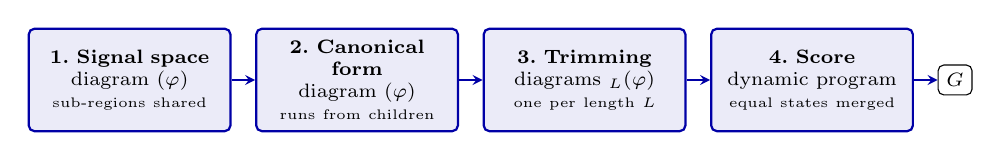
\begin{tikzpicture}[
    font=\scriptsize,
    stage/.style={draw=fastc, fill=fastc!8, thick, rounded corners=2pt,
                  text width=2.35cm, align=center, minimum height=1.3cm,
                  inner sep=3pt, anchor=west,
                  execute at begin node={\hyphenpenalty=10000\exhyphenpenalty=10000}},
    flow/.style={-stealth, semithick, fastc},
  ]
  % each box: stage name / what tabex_fast builds / how
  \node[stage] (f0) at (0,0)
    {\textbf{1.\ Signal space}\\ diagram $\Dg(\varphi)$\\ {\tiny sub-regions shared}};
  \node[stage] (f1) at ([xshift=\figgap]f0.east)
    {\textbf{2.\ Canonical form}\\ diagram $\Cg(\varphi)$\\ {\tiny runs from children}};
  \node[stage] (f2) at ([xshift=\figgap]f1.east)
    {\textbf{3.\ Trimming}\\ diagrams $\Cg_L(\varphi)$\\ {\tiny one per length $L$}};
  \node[stage] (f3) at ([xshift=\figgap]f2.east)
    {\textbf{4.\ Score}\\ dynamic program\\ {\tiny equal states merged}};
  \node[draw, rounded corners=2pt, inner sep=3pt, anchor=west] (g)
    at ([xshift=\figgap]f3.east) {$G$};

  \foreach \a/\b in {f0/f1, f1/f2, f2/f3, f3/g}
    \draw[flow] (\a) -- (\b);
\end{tikzpicture}
\caption{The four stages of \texttt{tabex\_fast}. Each computes exactly the
object the methodology of
Sections~\ref{sec:SignalSpace}--\ref{sec:MetricDefinition} defines, but stores
it more compactly.
(1)~The methodology evaluates the recursion $\Ev$ into a set of boxes whose
union is $\Sig(\varphi)$, and nested operators multiply boxes (about
$1.5\cdot10^{6}$ for $\mathsf{G}_{[0,16]}\mathsf{F}_{[0,4]}\chi$).
\texttt{tabex\_fast} evaluates the same recursion on a hash-consed decision
diagram, which stores each distinct sub-region once
(Lemma~\ref{lem:diag-sem}).
(2)~The methodology canonicalises by computing the runs of each axis and
keeping the products of runs that lie in the region; $\mathsf{F}_{[0,20]}\chi$
has $3^{21}-2^{21}$ such canonical boxes. \texttt{tabex\_fast} reads the runs
off the diagram's child nodes and relabels its edges by run. The resulting
diagram has exactly the canonical boxes as its paths, so they are counted
but never listed (Lemma~\ref{lem:arr-indep},
Proposition~\ref{prop:canon-diag}).
(3)~Instead of trimming each canonical box, \texttt{tabex\_fast} splits the
canonical diagram by trimmed length (Lemma~\ref{lem:trim}).
(4)~Eq.~\eqref{eq:OWSim} compares every canonical box of $\varphi$ with every
canonical box of $\vartheta$. \texttt{tabex\_fast} obtains the same best
matches with a dynamic program over the two diagrams, which merges partial
boxes that reach the same state (Theorem~\ref{thm:compat}).
Stages 1--3 run on each formula separately; only stage~4 reads both, and it
returns $G(\varphi,\vartheta)$.}
\label{fig:pipelines}
\end{figure}
